\documentclass{article}

\usepackage{assign}

\setcoursetitle{CS698X: Topics in Probabilistic Modelling and Inference}
\setassigncode{2}
\setstartnewpage{TRUE}

\begin{document}
\makeheader

\begin{question}

	Since $p(\vx \pipe \theta)$ is a Guassian with fixed covariance matrix, we can write
	\begin{align*}
		p(\vx \pipe \theta)	\eq	p(\vx \pipe \vmu)	\eq	\para{\frac{1}{\para{2 \pi}^D \abs{\vSigma}}}^{1 / 2} \cdot \texp{\frac{1}{2} \tr{\para{\vx - \vmu}} \vSigma^{-1} \para{\vx - \vmu}}
	\end{align*}

	We can therefore compute $g(.)$ as follows
	\begin{align*}
		g(\vx, \theta)	&\eq	\nabla_\theta \log{p(\vx \pipe \theta)}	\eq	\nabla_\vmu \log{p(\vx \pipe \vmu)} \\
		&\eq	\nabla_\vmu \brac{\frac{1}{2} \tr{\para{\vx - \vmu}} \vSigma^{-1} \para{\vx - \vmu} - \frac{D}{2} \log{2 \pi} - \frac{1}{2} \log{\abs{\vSigma}}} \\
		&\eq	\vSigma^{-1} \para{\vx - \vmu}
	\end{align*}

	For $\vF$, we can write
	\begin{align*}
		\vF	&\eq	\E[p(\vx \spipe \vmu)]{g(\vx, \theta) \tr{g(\vx, \theta)}} \\
		&\eq	\int_{\bR^D} g(\vx, \theta) \tr{g(\vx, \theta)} p(\vx \pipe \theta) \id \vx \\
		&\eq	\para{\frac{1}{\para{2 \pi}^D \abs{\vSigma}}}^{1 / 2} \int_{\bR^D} \vSigma^{-1} \para{\vx - \vmu} \tr{\para{\vx - \vmu}} \vSigma^{-1} \texp{\frac{1}{2} \tr{\para{\vx - \vmu}} \vSigma^{-1} \para{\vx - \vmu}} \id \vx
	\end{align*}

	Abusing the fact that $\vSigma$ is a constant, using equation (61) from \cite{matrix-cookbook}, we write this as
	\begin{align*}
		\vF	&\eq	\para{\frac{1}{\para{2 \pi}^D \abs{\vSigma}}}^{1 / 2} \int_{\bR^D} 2 \derp{\texp{\frac{1}{2} \tr{\para{\vx - \vmu}} \vSigma^{-1} \para{\vx - \vmu}}}{\vSigma} \id \vx \\
		&\eq	2 \para{\frac{1}{\para{2 \pi}^D \abs{\vSigma}}}^{1 / 2} \derp{\int_{\bR^D} \texp{\frac{1}{2} \tr{\para{\vx - \vmu}} \vSigma^{-1} \para{\vx - \vmu}} \id \vx}{\vSigma}
	\end{align*}

	The second equality is because the integral is over $\vx$ which is independent of $\vSigma$. Since the term within the integral is proportional to that of a gaussian, we can write it as
	\begin{align*}
		\vF	&\eq	2 \para{\frac{1}{\para{2 \pi}^D \abs{\vSigma}}}^{1 / 2} \derp{\sqrt{\para{2 \pi}^D \abs{\vSigma}}}{\vSigma} \\
		&\eq	\vSigma^{-1}
	\end{align*}

	The last equality follows from equation (49) from \cite{matrix-cookbook}

	Therefore, we can now write the final form of the kernel similarity
	\begin{align*}
		\kappa(\vx, \vx')	\eq	\tr{g(\vx, \theta)} \vF^{-1} g(\vx', \theta)
	\end{align*}
	Substituting from the terms of $g(.)$ and $\vF$, we get
	\answer[0.7\textwidth]{
		\begin{equation}
			\tag{a}
			\kappa(\vx, \vx')	\eq	\tr{\para{\vx - \vmu}}\,\vSigma^{-1}\,\para{\vx' - \vmu}
		\end{equation}
	}

	In case the covariance matrix is an identity matrix, we have
	\answer[0.7\textwidth]{
		\begin{equation}
			\tag{b}
			\kappa(\vx, \vx')	\eq	\tr{\para{\vx - \vmu}} \para{\vx' - \vmu}
		\end{equation}
	}

	\begin{qsubsection}{Intuitive Meaning}

		Since $\vSigma^{-1}$ is a positive definitive square matrix, for some $\vU \in \bR^{N \times N}$, we can say $\vSigma^{-1} = \tr{\vU} \vU$. Therefore, replacing this in the kernel term, we have
		\begin{align*}
			\kappa(\vx, \vx')	&\eq	\tr{\para{\vx - \vmu}}\,\tr{\vU} \vU\,\para{\vx' - \vmu} \\
			&\eq	\dotp{\vU \para{\vx - \vmu}}{\vU \para{\vx' - \vmu}}
		\end{align*}

		We wish to see when the value of this kernel is maximum. Suppose if we limit the norms of $\para{\vx - \vmu}$ and $\para{\vx' - \vmu}$ to 1, \ie $\norm{\vx - \vmu} = 1 = \norm{\vx' - \vmu}$, then we can say that the dot product will be maximum when $\vU (\vx - \vmu) = \vU (\vx' - \vmu) \implies \vx = \vx'$.

		From this, we can infer that if the norms of $\vx - \vmu$ and $\vx' - \vmu$ are fixed, then the kernel value will be maximum when the angle between the vectors $\vx - \vmu$ and $\vx' - \vmu$ is the least, and will be minimum when the angle is the largest.

	\end{qsubsection}

\end{question}

\begin{question}

	Let us write the expression for $f(.)$ alternatively
	\begin{align*}
		g_n(\vx, y)	\eq	f(\vx - \vx_n, y - y_n)	\eq	\ND{
			\brac{
				\begin{matrix}
					\vx - \vx_n \\
					y - y_n
				\end{matrix}
			} \ \bigg|\ \vzero, \sigma^2\vI
		}
	\end{align*}

	Using gaussian properties, we can say that this is equivalent to
	\begin{align*}
		g_n(\vx, y)	\eq	\ND{
			\brac{
				\begin{matrix}
					\vx \\
					y
				\end{matrix}
			}
			\bigg| \brac{
				\begin{matrix}
					\vx_n \\
					y_n
				\end{matrix}
			}, \sigma^2 \vI
		}
	\end{align*}

	Hence, we can rewrite the joint distribution as
	\begin{align*}
		\prob{\vx, y}	\eq	\sum_{n = 1}^N g_n(\vx, y)
	\end{align*}

	In order to compute the conditional probability $\prob{y \pipe \vx}$, we first compute the marginal probability $\prob{\vx}$, which can be expressed as
	\begin{align*}
		\prob{\vx}	&\eq	\int_\bR \prob{\vx, y} \id y \\
		&\eq	\int_\bR \frac{1}{N} \sum_{n = 1}^N g_n(\vx, y) \id y \\
		&\eq	\frac{1}{N} \sum_{n = 1}^N \int_\bR g_n(\vx, y) \id y \\
	\end{align*}

	Since $g_n(.)$ is a multivariate gaussian, using properties of gaussian, we can say
	\begin{align*}
		\prob{\vx}	\eq	\frac{1}{N} \sum_{n = 1}^N \ND{\vx \pipe \vx_n, \sigma^2 \vI}
	\end{align*}

	Now, we can write the marginal as
	\begin{align*}
		\prob{y \pipe \vx}	&\eq	\frac{\prob{y, \vx}}{\prob{\vx}} \\
		&\eq	\frac{1}{N \prob{\vx}} \sum_{n = 1}^N g_n(\vx, y)
	\end{align*}

	We can write $g(.)$ as
	\begin{align*}
		g(\vx, y)	&\eq	\para{\frac{1}{2 \pi \sigma^2}}^{\para{D + 1} / 2} \texp{ -\frac{\sigma^2}{2}
			\tr{
				\brac{
					\begin{matrix}
						\vx - \vx_n \\
						y - y_n
					\end{matrix}
				}
			}
			\brac{
				\begin{matrix}
					\vx - \vx_n \\
					y - y_n
				\end{matrix}
			}
		} \\
		&\eq \para{\frac{1}{2 \pi \sigma^2}}^{\para{D + 1} / 2} \texp{- \frac{\para{y - y_n}^2}{2\sigma^2}} \texp{ -\frac{\tr{\para{\vx - \vx_n}} \para{\vx - \vx_n}}{2 \sigma^2}} \\
		&\eq \ND{y \pipe y_n, \sigma^2} \ND{\vx \pipe \vx_n, \sigma^2 \vI}
	\end{align*}

	Hence, we can write the marginal as a weighted sum of univariate gaussians, as
	\begin{align*}
		\prob{y \pipe \vx}	\eq	\sum_{n = 1}^N \frac{\ND{\vx \pipe \vx_n, \sigma^2 \vI}}{\sum_{n' = 1}^N \ND{\vx \pipe \vx_{n'}, \sigma^2 \vI}} \ND{y \pipe y_n, \sigma^2}
	\end{align*}

	Writing this in a simplified manner, we get
	\answer{
		\begin{align*}
			\prob{y \pipe \vx}	\eq	\sum_{n = 1}^N \mu_n \ND{y \pipe y_n, \sigma^2}
		\end{align*}
	}
	where
	\begin{align*}
		\mu_n	\eq	\frac{\ND{\vx \pipe \vx_n, \sigma^2 \vI}}{\sum_{n' = 1}^N \ND{\vx \pipe \vx_{n'}, \sigma^2 \vI}}
	\end{align*}
	are the mixture weights.

	\begin{qsubsection}{Mean of the conditional}

		\begin{align*}
			\E[y \spipe \vx]{y}	&\eq	\int_\bR \sum_{n = 1}^N \mu_n \ND{y \pipe y_n, \sigma^2} y \id y \\
			&\eq	\sum_{n = 1}^N \mu_n \cdot \E[\ND{y \spipe y_n, \sigma^2}]{y}
		\end{align*}
		\answer{
			\begin{align*}
				\tfunc{mean}{y \pipe \vx} &\eq	\sum_{n = 1}^N \mu_n y_n
			\end{align*}
		}

	\end{qsubsection}

	\begin{qsubsection}{Variance of the conditional}

		\begin{align*}
			\E[y \spipe \vx]{y^2} - \E[y \spipe y_n, \sigma^2]{y}^2 &\eq	\int_\bR \sum_{n = 1}^N \mu_n \ND{y \pipe y_n, \sigma^2} y^2 \id y - \para{\sum_{n = 1}^N \mu_n y_n}^2 \\
			&\eq	\sum_{n = 1}^N \mu_n \para{\sigma^2 + y_n^2} - \para{\sum_{n = 1}^N \mu_n y_n}^2
		\end{align*}
		\answer{
			\begin{align*}
				\tfunc{var}{y \pipe \vx}	&\eq	\sigma^2 + \sum_{n = 1} \mu_n y_n^2 - \para{\sum_{n = 1}^N \mu_n y_n}^2
			\end{align*}
		}

	\end{qsubsection}

\end{question}

\begin{question}

	\begin{qpart}{A}

		Following the procedure of Laplace Approximation, let us write the second order Taylor expansion of $\log{\prob{x \pipe a, b}}$

		Let $f(x) = \log{\tfunc{Gamma}{x \pipe a, b}}$, then for some $x_0$
		\begin{align*}
			f(x)	&\qapprox	f(x_0) + f'(x_0) (x - x_0) + \frac{1}{2} f''(x_0) (x - x_0)^2
		\end{align*}

		As discussed in class, it is simpler to choose $x_0$ such that $f'(x_0)$ is 0 and $f''(x_0)$ is negative. A suitable option for this is the mode of the distribution. The mode of the gamma distribution is $(a - 1) / b$. This exists iff $a > 1$.

		Suppose the mode is represented by $m$, therefore, if $a > 1$, we set $x_0 = m = (a - 1) / b$. Hence, we can write
		\begin{align*}
			f(x)	&\qapprox	f(m) + \frac{1}{2} f''(m) (x - m)^2
		\end{align*}

		We can compute the double derivative as follows
		\begin{align*}
			f''(x)	&\eq	\frac{d^2}{dx^2} f(x) \\
			&\eq	\frac{d}{dx} f'(x) \\
			&\eq	\frac{d}{dx} \para{\log{b^a} - \log{\Gamma(a)} + (a - 1) \log{x} - bx} \\
			&\eq	\frac{d}{dx} \para{\frac{a - 1}{x} - b} \\
			&\eq	- \frac{a - 1}{x^2}
		\end{align*}

		Therefore,
		\begin{align*}
			f''(m)	&\eq	- \frac{a - 1}{m^2} \\
			&\eq	- \frac{b^2}{a - 1}
		\end{align*}

		We can now write the approximation for the gamma distribution
		\begin{align*}
			\tfunc{Gamma}{x \pipe a, b}	&\eq	\texp{f(x)} \\
			&\qapprox	\texp{f(m) + \frac{1}{2} f''(m) (x - m)^2} \\
			&\eq	\texp{f(m)} \texp{- \frac{1}{2} \frac{b^2}{a - 1} (x - m)^2} \\
			&\qprop	\texp{- \frac{1}{2} \para{\frac{b^2}{a - 1}} (x - m)^2}
		\end{align*}

		Therefore, we can approximate $\tfunc{Gamma}{x \pipe a, b}$ with the gaussian $\ND{x \pipe \mu, \sigma^2}$ where,
		\answer{
			\begin{align*}
				\mu			\eq	m	\eq	\frac{a - 1}{b} \\
				\sigma^2	\eq	\frac{a - 1}{b^2}
			\end{align*}
		}

	\end{qpart}

	\begin{qpart}{B}

		Suppose we approximate $\tfunc{Gamma}{x \pipe a, b}$ with the gaussian $\ND{x \pipe \mu', {\sigma'}^2}$ such that
		\begin{align*}
			\mu'		&\eq	\tfunc{mean}{x} \\
			{\sigma'}^2	&\eq	\tfunc{var}{x}
		\end{align*}

		Therefore,
		\answer{
			\begin{align*}
				\mu'		&\eq	\frac{a}{b} \\
				{\sigma'}^2	&\eq	\frac{a}{b^2}
			\end{align*}
		}

		This, therefore, is equivalent to the gaussian obtained using Laplace Approximation if the value of $a$ is large, \ie $a \gg 1$.

	\end{qpart}

	\begin{qpart}{C}

		We can use the Laplace approximation of the Gamma distribution obtained in Part A to approximate the gaussian function as follows
		\begin{align*}
			\func{\widetilde{\Gamma}}{a}	\qapprox	\frac{b^a}{\ND{x \pipe \mu, \sigma^2}} x^{a - 1} \exp{-bx}
		\end{align*}

		Since the LHS is independent of both $b$ and $x$, we can set arbitrary values for both. For simplicity, we assume $b = 1$ and $x = \mu = (a - 1) / b$. Therefore,
		\answer{
			\begin{align*}
				\func{\widetilde{\Gamma}}{a}	\eq	\para{2 \pi \sigma^2}^{1 / 2} \mu^{a - 1} \exp{- \mu}
			\end{align*}
		}

		A Comparision plot of the real Gamma function, $\Gamma(.)$ and the approximated Gamma function, $\widetilde{\Gamma}(.)$ is shown in Figure \ref{fig:q3}

		\begin{figure}[h!]
			\centering
			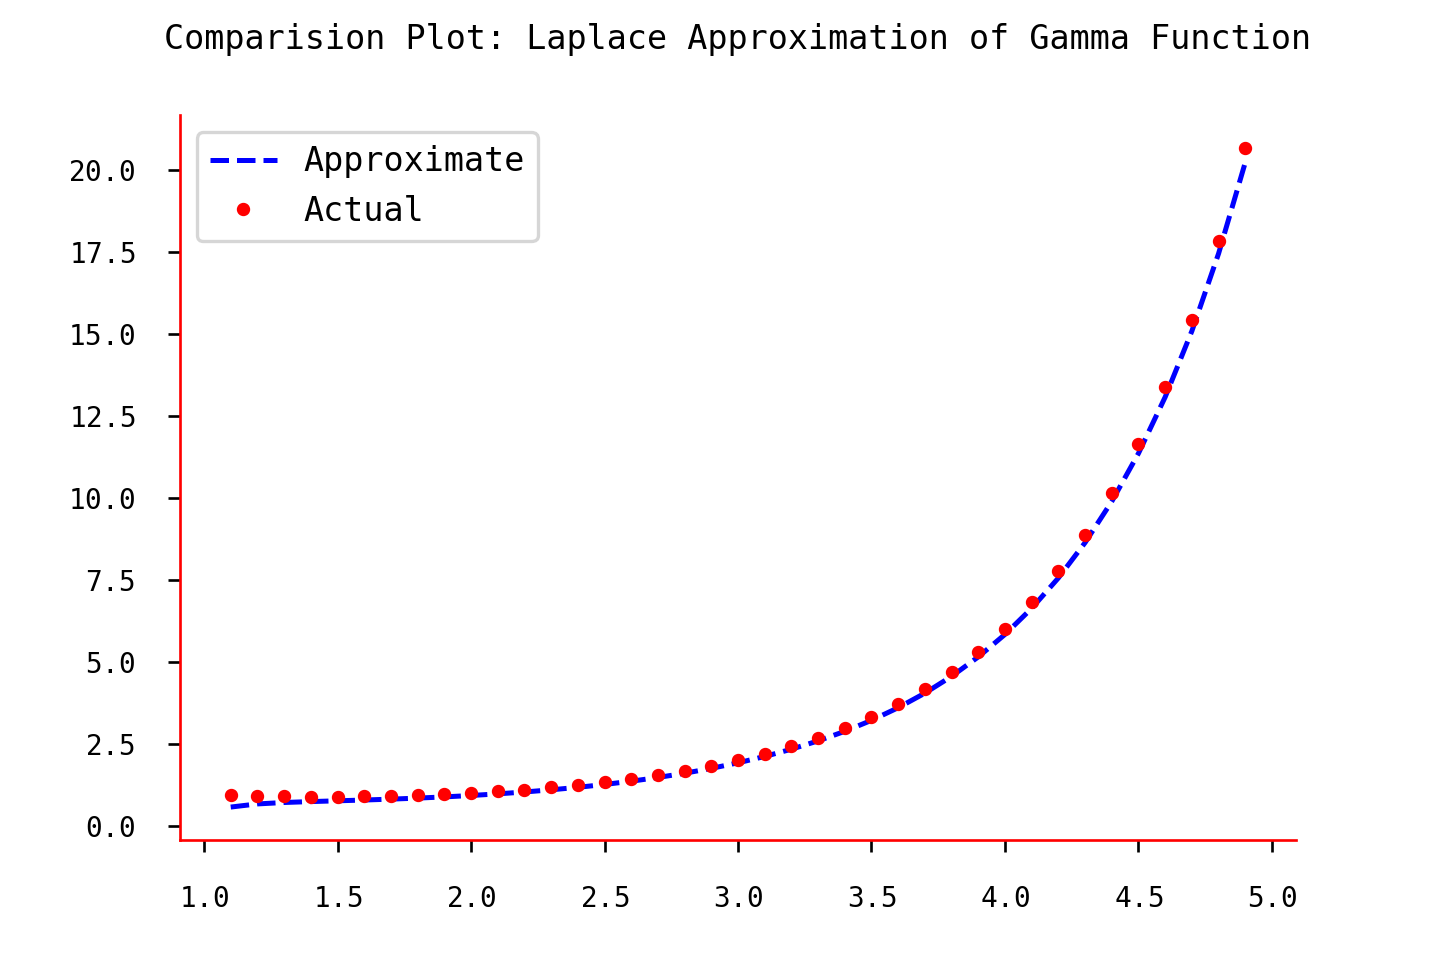
\includegraphics{plots/q3.png}
			\caption{$\Gamma(.)$ vs $\widetilde{\Gamma}(.)$}
			\label{fig:q3}
		\end{figure}

		It is clear from the figure that the approximation is indeed a good one, and there is small loss.

	\end{qpart}

\end{question}

\begin{question}

	The poisson distribution is written as
	\begin{align*}
		\prob{x \pipe \lambda}	\eq	\exp{- \lambda} \frac{\lambda^x}{\fact{x}}
	\end{align*}

	We can model a supervised learning problem as a Poisson distribution by mapping $\vx \in \bR^D$ to $\lambda$ as $\lambda = \tr{\vw} \vx$ for some $\vw \in \bR^D$.

	Therefore, we can write the likelihood as
	\begin{align*}
		\prob{y \pipe \vx, \vw}	\eq	\exp{-\tr{\vw} \vx} \frac{\para{\tr{\vw} \vx}^y}{\fact{y}}
	\end{align*}

	\begin{qsubsection}{Maximum Likelihood Estimation}

		We need to find the Log Likelihood ($\log{\prob{\vy \pipe \vX, \vw}}$) of the data, which is
		\begin{align*}
			\log{\prob{\vy \pipe \vX, \vw}}	&\eq	\log{\prod_{n = 1}^N \prob{y_n \pipe \vx_n, \vw}} \\
			&\eq	\sum_{n = 1}^N \log{\prob{y_n \pipe \vx_n, \vw}} \\
			&\eq	\sum_{n = 1}^N y_n \log{\tr{\vw} \vx} - \sum_{n = 1}^N \log{\fact{y_n}} - \tr{\vw} \para{\sum_{n = 1}^N \vx_n}
		\end{align*}

		Therefore the MLE estimate is given as
		\begin{align*}
			\vw_{\mt{MLE}}	&\eq	\argmax{\vw} \log{\prob{\vy \pipe \vX, \vw}} \\
			\implies 0		&\eq	\der{\log{\prob{\vy \pipe \vX, \vw}}}{\vw} \bigg|_{\vw_{\mt{MLE}}} \\
			\implies 0		&\eq	\sum_{n = 1}^{N} \frac{y_n}{\tr{\vw_{\mt{MLE}}} \vx_n} \vx_n - \sum_{n = 1}^N \vx_n
		\end{align*}

		This clearly does not have a closed solution. Therefore, we need iterative methods such as Gradient Descent or second order methods such as Newton's Method. Since this is an unconstrained optimization, we can use vanilla Gradient Descent for the MLE computation, which I have shown in \hyperlink{algo:1}{Algorithm 1}

		\begin{algo}[0.9\textwidth]{Gradient Descent for MLE}

			\bt{Result:} MLE Estimate of $\vw$, \ie $\vw_{\text{MLE}}$ \sbr

			\bt{Steps:}
			\begin{enumerate}
				\item Initialize the value of $\vw$ as $\vw^{(0)}$
				\item For $t = 1, 2 \dots T$ or until convergence, do
					\begin{align*}
						\nabla L(\vw^{(t - 1)})	&\eq	\sum_{n = 1}^N \para{1 - \frac{y_n}{\tr{\vw^{(t - 1)}} \vx_n}} \vx_n \\
						\vw^{(t)}				&\eq	\vw^{(t - 1)} - \eta_t \nabla L(\vw^{(t - 1)})
					\end{align*}
				\item Return $\vw^{(t')}$ where $t'$ corresponds to the last iteration.
			\end{enumerate}

		\end{algo}

	\end{qsubsection}

\end{question}

\begin{question}

	We follow the standard EM procedure.
	We first give the posterior probability of the latent variables $z$, represented as $\prob{z_n \pipe y_n, \vx_n, \vw}$.
	It is however easier to separate the cases when $y_n = 1$ or $y_n = 0$.
	\begin{align*}
		\prob{z_n \pipe y_n = 1, \vx_n, \vw}	&\eq	\prob{z_n \pipe z_n > 0, \vx_n, \vw} \\
	\end{align*}
	This is similar to the truncated gaussian distribution \citep{wiki-trunc-gauss}. Hence, we can directly write the expression of the pdf for this
	\begin{align*}
		\prob{z_n \pipe y_n = 1, \vx_n, \vw}	&\eq	\is{z_n > 0} \frac{\ND{z_n \spipe \tr{\vw} \vx_n, 1}}{1 - \vPhi(-\tr{\vw} \vx_n)}
	\end{align*}
	where $\vPhi(.)$ denotes the CDF function of the standard gaussian distribution.

	Similarly, we can write the expression in case $y_n = 0$
	\begin{align*}
		\prob{z_n \pipe y_n = 0, \vx_n, \vw}	&\eq	\is{z_n < 0} \frac{\ND{z_n \spipe \tr{\vw} \vx_n, 1}}{\vPhi(-\tr{\vw} \vx_n)}
	\end{align*}

	We can write this in a single expression as follows
	\begin{align*}
		\prob{z_n \pipe y_n, \vx_n, \vw}	\eq	\brac{y_n \frac{\is{z_n > 0}}{1 - \vPhi(-\tr{\vw} \vx_n)} + (1 - y_n) \frac{\is{z_n \le 0}}{\vPhi(-\tr{\vw} \vx_n)}} \ND{z_n \pipe \tr{\vw} \vx_n, 1}
	\end{align*}

	\begin{qsubsection}{Expectation Step}

		We can now write the Complete Data Likelihood as
		\begin{align*}
			\prob{\vy, \vz \pipe \vX, \vw}	&\eq	\prob{\vz \pipe \vy, \vX, \vw} \prob{\vy \pipe \vX, \vw} \\
			&\eq	\prod_{n = 1}^N \prob{z_n \pipe y_n, \vx_n, \vw} \prob{y_n \pipe x_n, \vw} \\
			&\eq	\prod_{n = 1}^N \ND{z_n \pipe \tr{\vw} \vx_n, 1} \brac{y_n \frac{\is{z_n > 0}}{1 - \vPhi(-\tr{\vw} \vx_n)} + (1 - y_n) \frac{\is{z_n \le 0}}{\vPhi(-\tr{\vw} \vx_n)}} \\&\hspace{5cm} \brac{y_n \para{1 - \vPhi(-\tr{\vw} \vx_n)} + (1 - y_n) \vPhi(-\tr{\vw} \vx_n)} \\
			&\eq	\prod_{n = 1}^N \ND{z_n \pipe \tr{\vw} \vx_n, 1} \brac{y_n\,\is{z_n > 0} + (1 - y_n)\,\is{z_n \le 0}}
		\end{align*}

		Therefore, the CLL is
		\begin{align*}
			\text{CLL}							&\eq	\sum_{n = 1}^N \log{y_n\,\is{z_n > 0} + (1 - y_n)\,\is{z_n \le 0}} - \frac{1}{2} \para{z_n - \tr{\vw} \vx_n}^2 - \frac{1}{2} \log{2 \pi} \\
			&\eq	\sum_{n = 1}^N y_n \log{\is{z_n > 0}} + (1 - y_n) \log{\is{z_n \le 0}} - \frac{1}{2} \para{z_n - \tr{\vw} \vx_n}^2 - \frac{1}{2} \log{2 \pi} \\
			\implies \E[\vz \spipe \vy]{\text{CLL}}	&\eq	\sum_{n = 1}^N y_n\,\E{\log{\is{z_n > 0}}} + (1 - y_n)\,\E{\log{\is{z_n \le 0}}} - \\ &\hspace{3cm} \frac{1}{2} \para{\E{z_n^2} - 2 \tr{\vw} \vx_n \E{z_n} + \para{\tr{\vw} \vx_n}^2} - \frac{1}{2} \log{2 \pi} \\
			&\eq	\sum_{n = 1}^N \frac{1}{2} \E{z_n^2} - \tr{\vw} \vx_n \E{z_n} + \frac{1}{2} \para{\tr{\vw} \vx_n}^2 - \frac{1}{2} \log{2 \pi}
		\end{align*}

		The last equality is obtained by analyising the expectations separately for the cases $y_n = 1$ and $y_n = 0$. We now compute the expectations required to completely express the $\E{\text{CLL}}$. These expectations, however, are computed with respected to a known (old) value of $\vw$, and are expressed as follows
		\begin{align*}
			\E[z_n \spipe y_n = 1]{z_n}		&\eq	\tr{\vw^{(\text{old})}} \vx_n + \frac{\func{\phi}{- \tr{\vw^{(\text{old})}} \vx_n}}{1 - \func{\vPhi}{- \tr{\vw^{(\text{old})}} \vx_n}} \\
			\E[z_n \spipe y_n = 0]{z_n}		&\eq	\tr{\vw^{(\text{old})}} \vx_n - \frac{\func{\phi}{- \tr{\vw^{(\text{old})}} \vx_n}}{\func{\vPhi}{- \tr{\vw^{(\text{old})}} \vx_n}} \\
			\implies \E[z_n \spipe y_n]{z_n}		&\eq	\tr{\vw^{(\text{old})}} \vx_n + \func{\phi}{- \tr{\vw^{(\text{old})}} \vx_n} \para{\frac{1}{1 - \func{\vPhi}{- \tr{\vw^{(old)}} \vx_n}}}^{y_n} \para{\frac{-1}{\func{\vPhi}{- \tr{\vw^{(old)}} \vx_n}}}^{1 - y_n}
		\end{align*}

		\begin{note}
			We do not need $\E{z_n^2}$ as it will not partake in the Maximization step (since it is constant with respect to $\vw$). Therefore, I have skipped its computation
		\end{note}

		Therefore, we can write the final expression of $\E{\text{CLL}}$ as follows
		\answer[0.7\textwidth]{
			\begin{align*}
				\E{\text{CLL}}		&\eq	\sum_{n = 1}^N \frac{1}{2} \E{z_n^2} - \tr{\vw} \vx_n \E{z_n} + \frac{1}{2} \para{\tr{\vw} \vx_n}^2 - \frac{1}{2} \log{2 \pi}
			\end{align*}
		}
		where $\phi(.)$ and $\vPhi(.)$ are the pdf and the cdf functions (respectively) of the standard gaussian distribution, and the expectation terms are as given in the previous equations.

	\end{qsubsection}

	\begin{qsubsection}{Maximization Step}

		Now, we can do MLE for the parameters by maximising the $\E{\text{CLL}}$ as in the standard EM Algorithm
		\begin{align*}
			\vw_{\text{MLE}}	&\eq	\argmax{\vw} \E{\text{CLL}} \\
		\end{align*}

		We need to differentiate this and equate to 0 for the desired MLE solution.
		\begin{align*}
			0	&\eq	\derp{\E{\text{CLL}}}{\vw} \bigg|_{\vw = \vw_{\text{MLE}}} \\
			&\eq	\sum_{n = 1}^N \para{\tr{\vw_{\text{MLE}}} \vx_n} \vx_n - \E{z_n} \vx_n \\
			&\eq	\tr{\vX} \vX \vw_{\text{MLE}} - \tr{\vX}\,\E{\vz}
		\end{align*}

		Therefore, we can write
		\answer{
			\begin{align*}
				\vw_{\text{MLE}}	&\eq	\para{\tr{\vX} \vX}^{-1} \tr{\vX}\,\E{\vz}
			\end{align*}
		}
		where
		\begin{align*}
			\E{\vz}	\eq \tr{\brac{\E[z_1 \spipe y_1]{z_1}, \E[z_2 \spipe y_2]{z_2} \dots \E[z_N \spipe y_N]{z_N}}}
		\end{align*}

	\end{qsubsection}

	We can write the complete EM algorithm as given in \hyperlink{algo:2}{Algorithm 2}

	\begin{algo}[0.9\textwidth]{EM Algorithm for Binary Classification as LVM}

		\bt{Result:} Posterior Distribution $\prob{\vz \pipe \vy, \vX, \vw}$, MLE estimate $\vw_{\text{MLE}}$ \sbr

		\bt{Steps:}

		\begin{enumerate}
			\item Initialize the value of $\vw$ as $\vw^{(0)}$
			\item For t = 1, 2 \dots T or until convergence, do
				\begin{enumerate}
					\ditem[E Step:]
						Given $\vw^{(t - 1)}$, compute the posteriors as
						\begin{align*}
							\qforall n \in \brac{N}, \quad \vPhi_n	&\eq	\func{\vPhi}{-\tr{\vw^{(t - 1)}} \vx_n} \\
							\qforall n \in \brac{N}, \quad \prob{z_n^{(t)} \pipe y_n, \vx_n, \vw^{(t - 1)}}	&\eq	\para{\frac{\is{z_n > 0}}{1 - \vPhi_n}}^{y_n} \para{\frac{\is{z_n \le 0}}{\vPhi_n}}^{(1 - y_n)} \\
							&\hspace{4cm}\ND{z_n^{(t)} \pipe \tr{\vw^{(t - 1)}} \vx_n, 1}
						\end{align*}
						Compute the expectation of $\vz$ as
						\begin{align*}
							\qforall n \in \brac{N}, \quad \E[z_n \spipe y_n]{z_n}		&\eq	\tr{\vw^{(\text{t - 1})}} \vx_n + \func{\phi}{- \tr{\vw^{(\text{t - 1})}} \vx_n} \para{\frac{1}{1 - \vPhi_n}}^{y_n} \para{-\frac{1}{\vPhi_n}}^{1 - y_n} \\
							\E{\vz}	&\eq \tr{\brac{\E[z_1 \spipe y_1]{z_1}, \E[z_2 \spipe y_2]{z_2} \dots \E[z_N \spipe y_N]{z_N}}}
						\end{align*}
					\ditem[M Step:]

						Compute the MLE solution of $\vw$ as
						\begin{align*}
							\vw^{(t)}	\eq	\para{\tr{\vX} \vX}^{-1} \tr{\vX}\,\E{\vz}
						\end{align*}
				\end{enumerate}
			\item Return $\prob{\vz \pipe \vy, \vX, \vw} = \prod_{n = 1}^N \prob{z_n^{(t')} \pipe y_n, \vX, \vw^{(t' - 1)}}$ and $\vw_{\text{MLE}} = \vw^{(t')}$
		\end{enumerate}

	\end{algo}

	\begin{note}
		It might not be possible to compute the values of $\func{\vPhi}{\tr{\vw} \vx_n}$ and therefore, we might need to approximate this as well using standard approximation techniques.
	\end{note}

\end{question}

\begin{question}

	\def\opi{\vpi^{\text{(old)}}}
	\def\oW{\vW^{\text{(old)}}}
	\def\obeta{\beta^{\text{(old)}}}
	\def\ovbeta{\para{\beta^{\text{(old)}}}^{-1}}

	\def\mleW{\vW_{\text{MLE}}}
	\def\mlebeta{\vbeta_{\text{MLE}}}
	\def\mlepi{\vpi_{\text{MLE}}}

	It is difficult to model $\prob{\vz_n \pipe \vx_n}$, not because it is intractable (since $\vz$ is from a discrete distribution), but becausing computing the posterior (at least accurately) would take $\bigO{2^K}$ time. This is not practical for large values of $K$, therefore, we will try to approximate the expectation step. To be more precise, we will approximate $\E{\vz_n \pipe \vx_n}$. First, it is better to actually compute $\E{\text{CLL}}$, assuming we know $\E{\vz_n \pipe \vx_n}$.

	\begin{align*}
		\prob{\vX, \vZ \pipe \vW, \beta}	&\eq	\prob{\vX \pipe \vZ, \vW, \beta} \cdot \prob{\vZ \pipe \vpi} \\
		&\eq	\prod_{n = 1}^N \set{\prob{\vx_n \pipe \vz_n, \vW, \beta} \prod_{k = 1}^K \prob{\z_{nk} \pipe \pi_k}} \\
	\end{align*}
	We know the forms of all these terms, and therefore write the CLL as follows,
	\begin{align*}
		\implies \text{CLL}	&\eq	\sum_{n = 1}^N \set{\frac{\beta}{2} \tr{\para{\vx_n - \vW \vz_n}} \para{\vx_n - \vW \vz_n} + \sum_{k = 1}^K \set{z_{nk} \log{\pi_k} + \para{1 - z_{nk}} \log{1 - \pi_k}}} + \mt{constants}
	\end{align*}

	We can now take the expectation of this ($\E{\text{CLL}}$) with respect to the distribution $\vZ \pipe \vX, \oW, \obeta, \opi$. The problem, as discussed earlier, is that the computation of the posterior probability will take $\bigO{2^K}$ time. Therefore, we choose to sample a set of values of $\vZ \pipe \vX$, and use Monte Carlo estimation for the expectations. My proposed solution for this is to use Gibbs Sampling, as there is conditional conjugacy in our case, which can be seen as below
	\begin{align*}
		\prob{z_{nk} \pipe \vx_n, \vz_{-nk}, \vW, \beta, \vpi}	&\eq	\prob{\vx_n \pipe z_{nk}, \vz_{-nk}, \vW, \beta} \prob{z_{nk} \pipe \vz_{-nk}, \vpi} \\
		&\eq	\prob{\vx_n \pipe z_{nk}, \vz_{-nk}, \vW, \beta} \prob{z_{nk} \pipe \pi_k} \\
		&\eq 	\ND{\vx_n \pipe \vW \vz_n, \beta^{-1} \vI} \tfunc{Bernoulli}{z_{nk} \pipe \pi_k} \\
		&\qprop	\texp{\frac{\beta}{2} \tr{\para{\vx_n - \vW \vz_n}} \para{\vx_n - \vW \vz_n}} \pi_k^{z_{nk}} (1 - \pi_k)^{(1 - z_{nk})}
	\end{align*}

	We can ignore all terms that are independent of, as we only need to analyse the form of the distribution.

	We can write $\vW \vz_n = \sum_{k' = 1}^K \vw_{k'} z_{nk'}$. Define $\vx_{-nk} = \vx_n - \sum_{\overset{k' = 1}{k' \ne k}}^K z_{nk'} \vw_{k'}$, then we can write
	\begin{align*}
		\prob{z_{nk} \pipe \vx_n, \vz_{-nk}, \vW, \beta, \vpi}	&\qprop	\texp{\frac{\beta}{2} \brac{z_{nk}^2 \tr{\vw_k} \vw_k - 2 z_{nk} \tr{\vx_{-nk}} \vw_k}} \para{\frac{\pi_k}{1 - \pi_k}}^{z_{nk}}
	\end{align*}
	Since $z_{nk} \in \set{0, 1}$, $z_{nk}^2 = z_{nk}$. Therefore,
	\begin{align*}
		\prob{z_{nk} \pipe \vx_n, \vz_{-nk}, \vW, \beta, \vpi}	&\qprop	\para{\texp{\frac{\beta}{2} \brac{\tr{\vw_k} \vw_k - 2\,\tr{\vx_{-nk}} \vw_k}} \frac{\pi}{1 - \pi_k}}^{z_{nk}}
	\end{align*}
	This represents a Bernoulli. Hence, we can say there is conditional conjugacy. Therefore, we can write the conditional posterior as follows
	\begin{align*}
		\prob{z_{nk} \pipe \vx_n, \vz_{-nk}, \vW, \beta, \vpi}	&\eq	\pi'_k^{z_{nk}} (1 - \pi'_k)^{(1 - z_{nk})}
	\end{align*}
	where
	\begin{align*}
		\pi'_k	\eq	\frac{\texp{\frac{\beta}{2} \tr{\para{\vw_k - 2 \vx_{-nk}}} \vw_k} \pi_k}{1 + \pi \para{\texp{\frac{\beta}{2} \tr{\para{\vw_k - 2 \vx_{-nk}}} \vw_k} - 1}}
	\end{align*}

	Therefore, we can perform Gibbs Sampling to compute $M$ samples of $\vZ$ and approximate $\E{\text{CLL}}$ using (unweighted) Monte Carlo estimation. The Gibbs Sampling algorithm is given in Algorithm \hyperlink{algo:3}{3}

	\begin{algo}[0.9\textwidth]{Gibbs Sampling for Latent Variables, $\vZ$}

		\bt{Result:} Sample set, $\cS = \set{\vZ^{(1)}, \vZ^{2} \dots \vZ^{M}}$ \sbr

		\bt{Steps:}
		\begin{enumerate}
			\item Initialize the zero\tth sample as $\vZ^{(0)}$
			\item For $m = 1, 2 \dots M$
				\begin{enumerate}
					\item For all $k \in \brac{K}$,
						\begin{align*}
							\pi'_k	\eq	\frac{\texp{\frac{\beta}{2} \tr{\para{\vw_k - 2 \vx_{-nk}}} \vw_k} \pi_k}{1 + \pi \para{\texp{\frac{\beta}{2} \tr{\para{\vw_k - 2 \vx_{-nk}}} \vw_k} - 1}}
						\end{align*}
					\item For all $n \in \brac{N}, k \in \brac{K}$, sample $z_{nk}^{m}$ as
						\begin{align*}
							z_{nk}^{(m)}	\qsim	\tfunc{Bernoulli}{\pi'_k}
						\end{align*}
				\end{enumerate}
			\item Return $\cS = \set{\vZ^{(1)}, \vZ^{(2)} \dots \vZ^{(M)}}$
		\end{enumerate}

	\end{algo}

	\begin{qsubsection}{Expectation Step}

		Suppose we can call the above algorithm (Algorithm \hyperlink{algo:3}{3}) as $\ffunc{GibbsSampler}{\oW, \obeta, \opi}$. Then we can estimate $\E{\text{CLL}}$ as follows
		\begin{align*}
			\E{\text{CLL}}	&\qapprox	\sum_{\vZ \in \cS}\ \sum_{n = 1}^N \bigg\{ \frac{D}{2} \log{\beta} - \frac{\beta}{2} \tr{\para{\vx_n - \vW \vz_n}} \para{\vx_n - \vW \vz_n} \ + \dots\\
			&\hspace{35mm}\dots + \sum_{k = 1}^K \set{z_{nk} \log{\pi_k} + (1 - z_{nk}) \log{1 - \pi_k}} \bigg\} + \mt{constants}
		\end{align*}
		where $\cS = \ffunc{GibbsSampler}{\oW, \obeta, \opi}$.

	\end{qsubsection}

	\begin{qsubsection}{Maximization Step}

		We can now maximize the $\E{\text{CLL}}$ over the parameters, namely $\set{\vW, \vpi}$. Hence, we can write this as
		\begin{align*}
			\set{\vW_{\text{MLE}}, \beta_{\text{MLE}}, \vpi_{\text{MLE}}}	\eq	\argmax{\set{\vW, \beta, \vpi}} \E{\text{CLL}}
		\end{align*}

		Using standard MLE approach, we get
		\begin{enumerate}
				\ditem[MLE of $\vpi$]
				\begin{align*}
					0	&\eq	\derp{\E{\text{CLL}}}{\pi_k}\\
					\implies \pi_{\text{k, MLE}}	&\eq	\frac{1}{N \cdot \abs{\cS}} \sum_{\vZ \in \cS}\ \sum_{n = 1}^N {z_{nk}} \\
					&\eq	\frac{1}{N} \sum_{n = 1}^N \E{z_{nk}} \\
					&\eq	\frac{1}{N} \sum_{n = 1}^N \E{\vz_n}_k
				\end{align*}
				\ditem[MLE of $\vW$]
				Similarly, for $\vW$
				\begin{align*}
					0	&\eq	\derp{\E{\text{CLL}}}{\vW} \bigg|_{\vW = \vW_{\text{MLE}}}\\
					\implies 0	&\eq	\sum_{\vZ \in \cS}\ \sum_{n = 1}^N \set{\vx_n \tr{\vz_n} - \vW_{\text{MLE}}\ \vz_n \tr{\vz_n}}\\
					\implies \vW_{\text{MLE}}	&\eq	\para{\sum_{\vZ \in \cS}\ \sum_{n = 1}^N \vx_n \tr{\vz_n}} \para{\sum_{\vZ \in \cS}\ \sum_{n = 1}^N \vz_n \tr{\vz_n}}^{-1} \\
					\implies \vW_{\text{MLE}}	&\eq	\para{\sum_{n = 1}^N \vx_n \tr{\E{\vz_n}}} \para{\sum_{n = 1}^N \E{\vz_n \tr{\vz_n}}}^{-1} \\
					\implies \vW_{\text{MLE}}	&\eq	\para{\sum_{n = 1}^N \vx_n \tr{\E{\vz_n}}} \E{\vZ \tr{\vZ}}^{-1}
				\end{align*}
				\ditem[MLE of $\beta$]
				\begin{align*}
					0	&\eq	\derp{\E{\text{CLL}}}{\beta} \bigg|_{\beta = \beta_{\text{MLE}}} \\
					\implies 0	&\eq	\sum_{\vZ \in \cS}\ \sum_{n = 1}^N \set{\frac{D}{2 \beta} - \frac{1}{2} \tr{\para{\vx_n - \vW \vz_n}} \para{\vx_n - \vW \vz_n}} \\
					\implies \beta_{\text{MLE}}	&\eq	N D \cdot \abs{\cS} \para{\sum_{\vZ \in \cS} \sum_{n = 1}^N \tr{\para{\vx_n - \vW \vz_n}} \para{\vx_n - \vW \vz_n}}^{-1} \\
					\implies \beta_{\text{MLE}}	&\eq	N D \cdot \para{\sum_{n = 1}^N \E{\tr{\para{\vx_n - \vW \vz_n}} \para{\vx_n - \vW \vz_n}}}^{-1} \\
					\implies \beta_{\text{MLE}}	&\eq	N D \cdot \para{\sum_{n = 1}^N \set{\tr{\vx_n} \vx_n + - 2 \tr{\vx_n} \mleW \E{\vz_n} + \E{\tr{\vz_n} \tr{\mleW} \mleW \vz_n}}}^{-1} \\
					\implies \beta_{\text{MLE}}	&\eq	N D \cdot \para{\sum_{n = 1}^N \set{\tr{\vx_n} \vx_n + - 2 \tr{\vx_n} \mleW \E{\vz_n} + \trace{\E{\vz_n \tr{\vz_n}} \tr{\mleW} \mleW}}}^{-1}
				\end{align*}
		\end{enumerate}

	\end{qsubsection}

	I have generalised the complete algorithm in Algorithm \hyperlink{algo:4}{4}

	\begin{algo}[0.9\textwidth]{EM Algorithm for Subset Sum Model}

		\bt{Result:} Posterior Distribution $\prob{\vZ \pipe \vX, \vW, \beta, \vpi}$, MLE estimates $\set{\vw_{\text{MLE}}, \beta_{\text{MLE}}, \vpi_{\text{MLE}}}$ \sbr

		\bt{Steps:}

		\begin{enumerate}
			\item Initialize the value of $\vw$ as $\vw^{(0)}$
			\item For t = 1, 2 \dots T or until convergence, do
				\begin{enumerate}
					\ditem[E Step:]
					Given $\set{\vW, \beta, \vpi}^{(t - 1)}$, approximate the posterior as a set of samples from the posterior using Algorithm \hyperlink{algo:3}{3} \ie
						\begin{align*}
							\cS^{(t)} = \ffunc{GibbsSampler}{\vW^{(t - 1)}, \beta^{(t - 1)}, \vpi^{(t - 1)}} \sim \prob{\vZ \pipe \vW^{(t - 1)}, \beta^{(t - 1)}, \vpi^{(t - 1)}}
						\end{align*}
						Then approximate the expectations required as follows
						\begin{align*}
							\qforall n \in \brac{N}, \quad \E{\vz_n^{(t)}}			&\eq	\frac{1}{\abs{\cS}} \sum_{\vZ \in \cS} \vz_n \\
							\qforall n \in \brac{N}, \quad \E{\vz_n^{(t)} \tr{\vz_n^{(t)}}}	&\eq	\frac{1}{\abs{\cS}} \sum_{\vZ \in \cS} \vz_n \tr{\vz_n} \\
							\qforall n \in \brac{N}, \quad \E{\vZ^{(t)} \tr{\vZ}^{(t)}}		&\eq	\sum_{n = 1}^N \E{\vz_n \tr{\vz_n}}
						\end{align*}
					\ditem[M Step:]
						Compute the MLE solutions of $\set{\vW, \beta, \vpi}$ as
						\begin{align*}
							\qforall k \in \brac{K}, \quad \pi_k^{(t)}	&\eq	\frac{1}{N} \sum_{n = 1}^N \E{\vz_n^{(t)}}_k \\
							\vW^{(t)}									&\eq	\para{\sum_{n = 1}^N \vx_n \tr{\E{\vz_n^{(t)}}}} \E{\vZ^{(T)} \tr{\vZ^{(t)}}}^{-1} \\
							\para{\beta^{(t)}}^{-1}						&\eq	\frac{1}{N D} \sum_{n = 1}^N \set{\tr{\vx_n} \vx_n + - 2 \tr{\vx_n} \vW^{(t)} \E{\vz_n^{(t)}} + \trace{\E{\vz_n^{(t)} \tr{\vz_n^{(t)}}} \tr{\vW^{(t)}} \vW^{(t)}}}
						\end{align*}
				\end{enumerate}
			\item Return $\prob{\vZ \pipe \vX, \vW, \beta, \vpi}$ as a set of samples $\cS$, and $\set{\vW, \beta, \vpi}_{\text{MLE}} = \set{\vW, \beta, \vpi}^{(t')}$, where $t'$ can represent the best value, computed over the average values or the last value ($T$), as per our choice.
		\end{enumerate}

	\end{algo}

\end{question}

\bibliographystyle{plainnat}
\bibliography{assign2}

\end{document}
